\chapter{Inversion Results}\label{app:inversion_results}
\section{Latent Space Optimization}
During \gls{lso}, the losses for each of the 100~optimized latents were computed using a combination of context loss~($\Lambda_{context}$) and geological prior loss~($\Lambda_{prior}$) during each iteration. Figure~\ref{fig:appendix_post_lso_losses} showcases the total loss for each of the \gls{lso} runs.

\begin{figure}[htbp!]
    \centering
    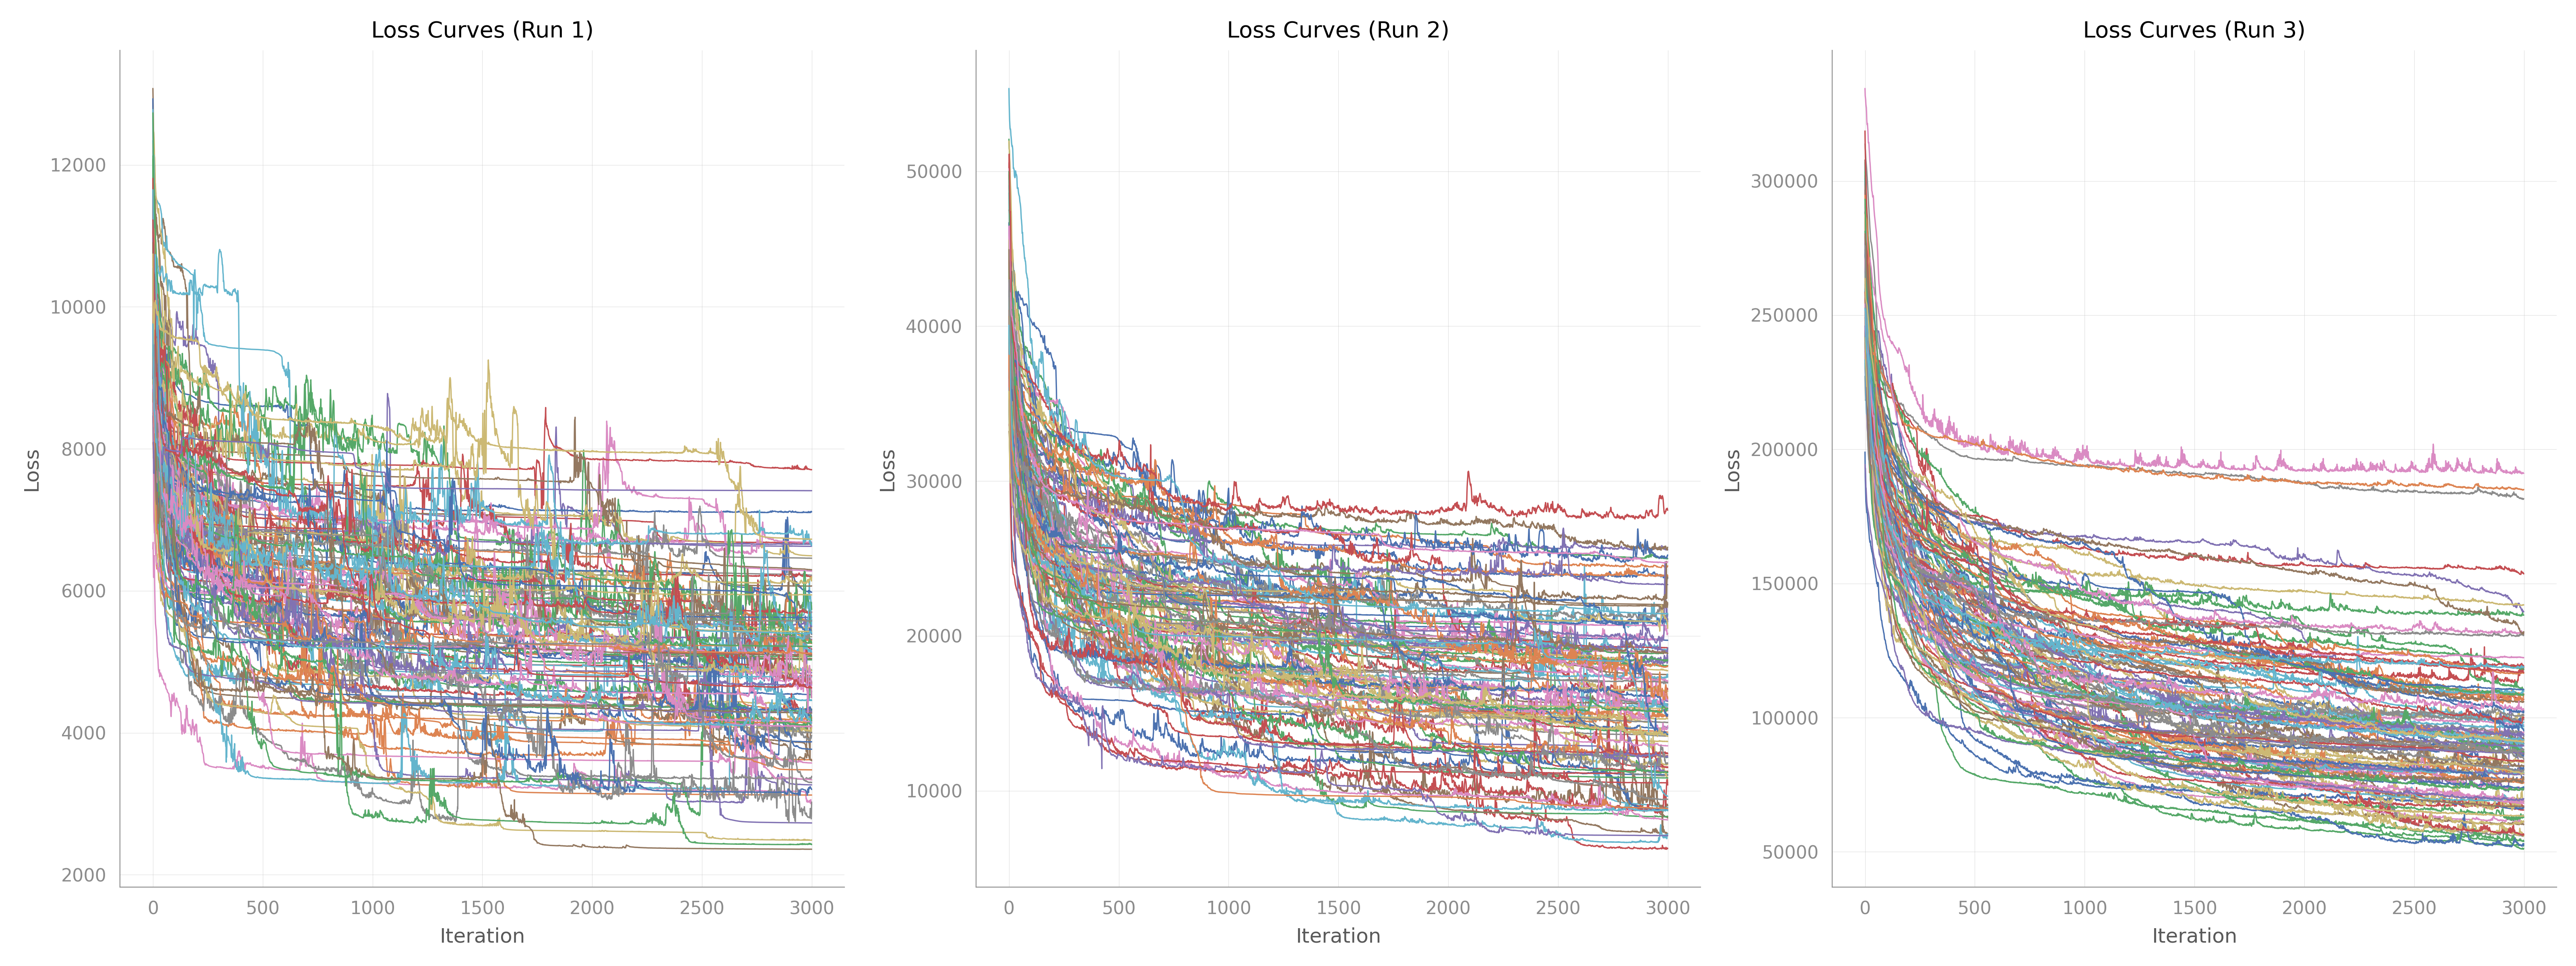
\includegraphics[width=0.99\linewidth]{figures/appendix/appendix_F/latent_space_optimization_loss.png}
    \caption{Loss curves of the different runs (Run 1: th = 1, Run 2: th= 2, Run 3: th = 5) over 3000 iterations. The total loss increases as the threshold increases from 1 to 5.}
    \label{fig:appendix_post_lso_losses}
\end{figure}

\section{Pivotal Tuning}
\begin{figure}[htbp!]
    \centering
    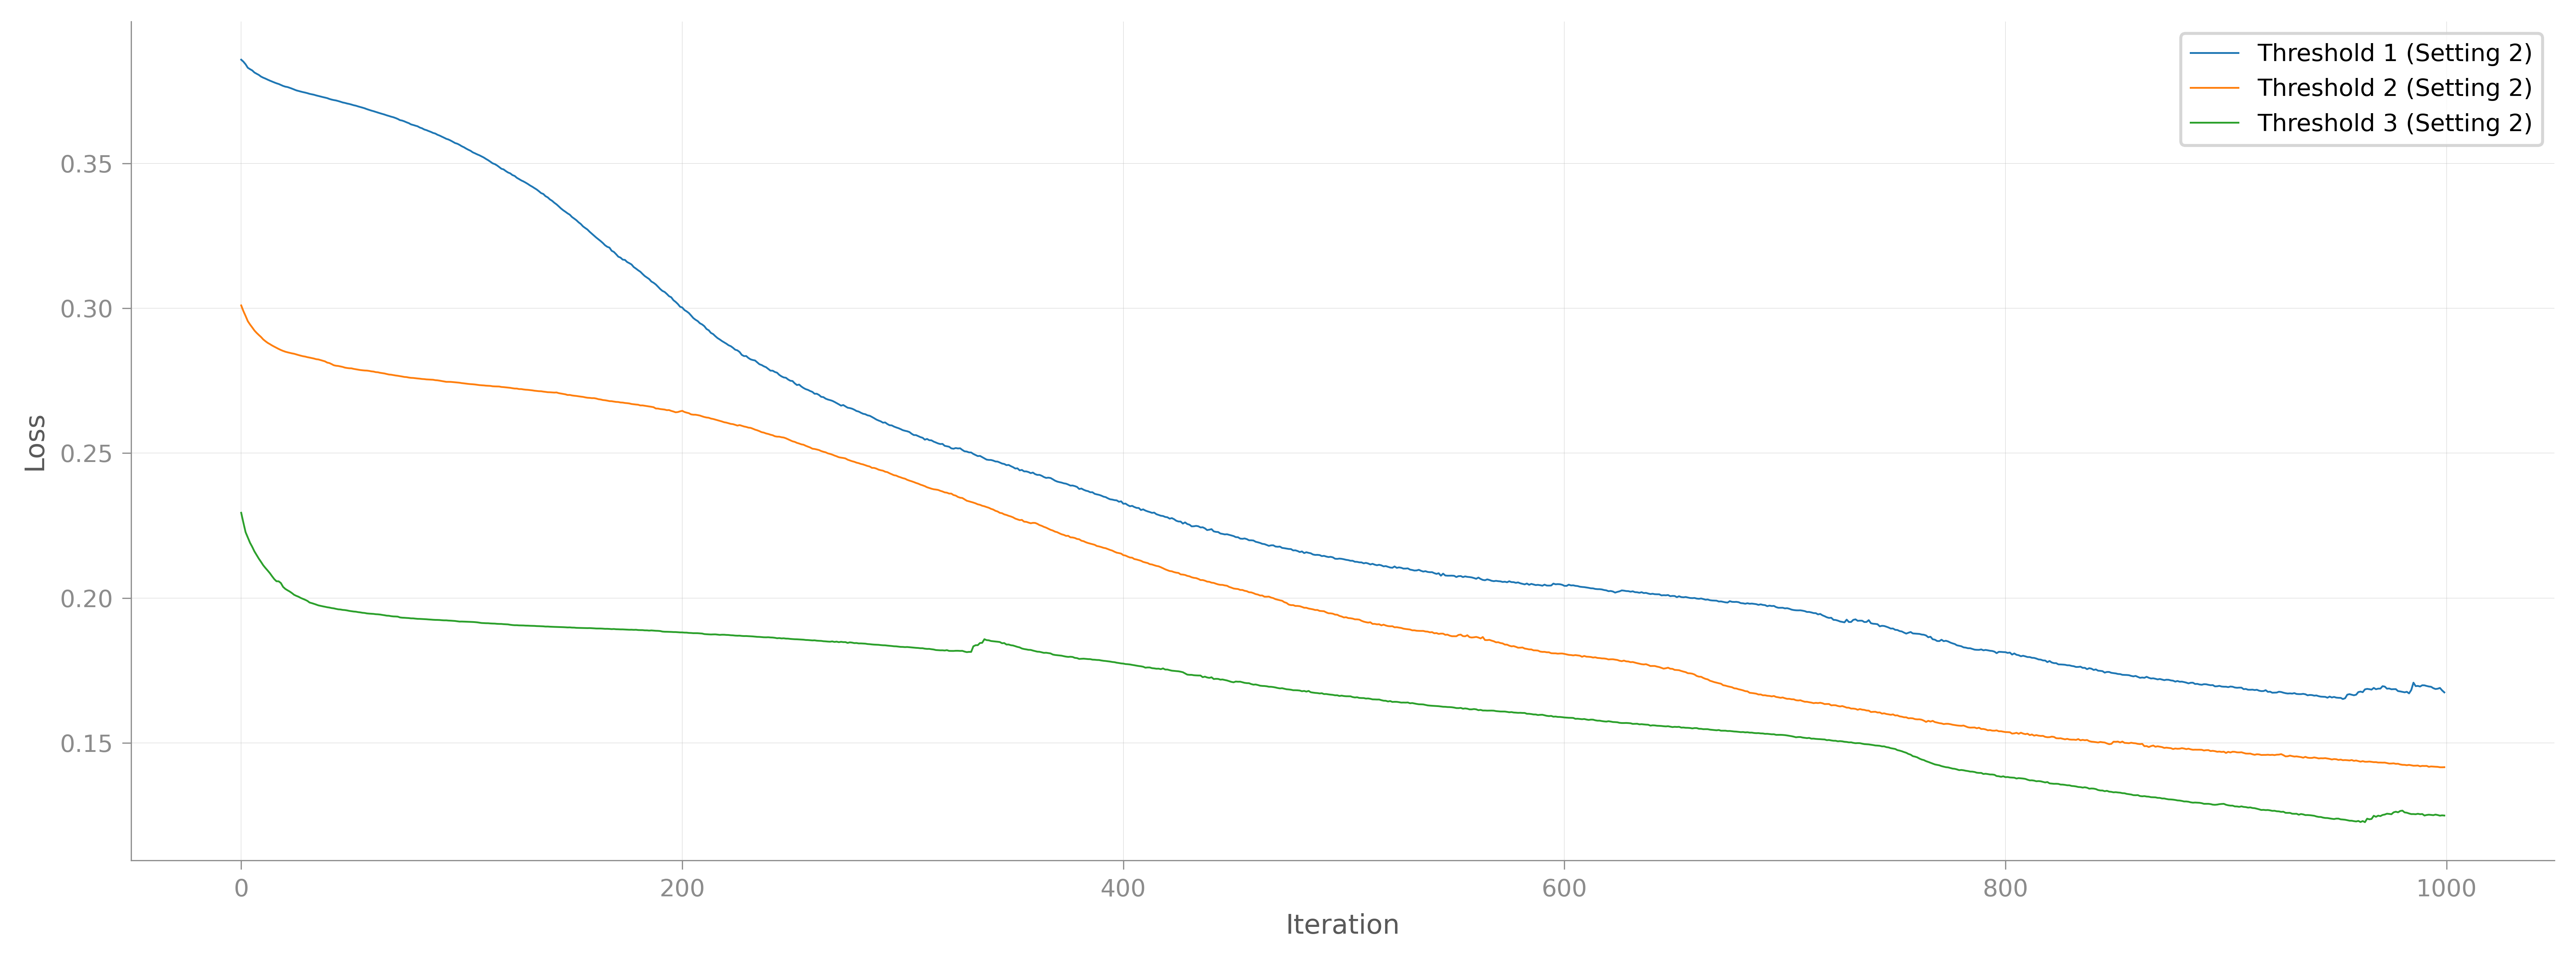
\includegraphics[width=0.99\linewidth]{figures/appendix/appendix_F/pivotal_tuning_loss.png}
    \caption{Loss curves of the pivotal tuning runs with different threshold values.}
    \label{fig:appendix_post_lso_losses}
\end{figure}